% =============================================================
% Capitulo 3 - Fotodeteccion y acondicionamiento de senales pulsadas
% =============================================================
\chapter{Fotodetección del láser}
\label{cap:fotodeteccion}

\section{Modelo del fotodiodo y amplificador de transimpedancia}
\label{sec:modelo_fotodiodo}

Un fotodiodo es un sensor óptico que genera una corriente o una tensión cuando la luz incide sobre la unión PN del semiconductor que lo compone, y se emplea habitualmente para detectar la presencia, la intensidad o el color de una señal luminosa \cite{hamamatsu2025}. Su comportamiento eléctrico se describe mediante el circuito equivalente de la Figura~\ref{fig:modelo_fotodiodo}, en el que la fotocorriente se representa como una fuente de corriente $I_L$ proporcional a la potencia luminosa incidente, en paralelo con un diodo ideal, la capacidad de juntura $C_j$ y la resistencia de derivación (\emph{shunt}) $R_{sh}$, y en serie con una resistencia $R_s$ \cite{hamamatsu2025}.

A partir de este circuito, la corriente de salida $I_O$ del fotodiodo resulta

\begin{equation}
  I_O = I_L - I_D - I' = I_L - I_S\left[\exp\!\left(\frac{q\,V_D}{k\,T}\right) - 1\right] - I'
  \label{eq:fotodiodo}
\end{equation}

\noindent donde $I_L$ es la corriente fotogenerada, $I_D$ la corriente del diodo, $I_S$ la corriente de saturación inversa, $I'$ la corriente que circula por $R_{sh}$, $V_D$ la tensión sobre el diodo, $q$ la carga del electrón, $k$ la constante de Boltzmann y $T$ la temperatura absoluta del fotodiodo \cite{hamamatsu2025}.

\begin{figure}[!h]
  \centering
  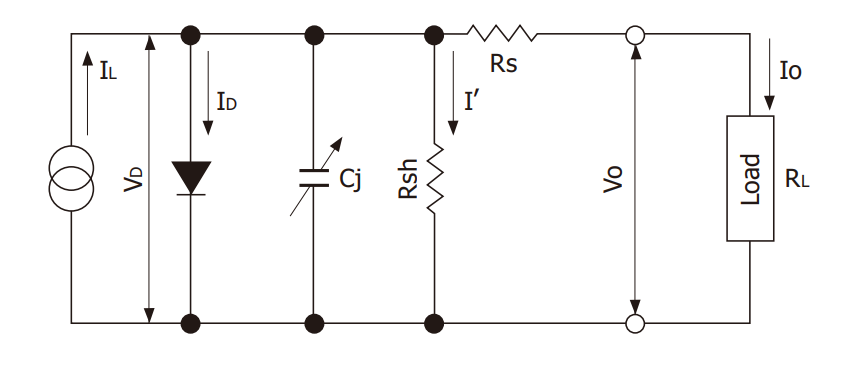
\includegraphics[width=0.7\textwidth]{figuras/3_circuitoequivalente.png}
  \caption{Circuito equivalente del fotodiodo con fuente de corriente. (Fuente: Hamamatsu \cite{hamamatsu2025}).}
  \label{fig:modelo_fotodiodo}
\end{figure}

\subsection{Respuesta temporal y detección del pico}
\label{subsec:respuesta_temporal}

Dado que en el sistema HSRL de Pilar el láser host emite pulsos de muy corta duración (entre 4~ns y 6~ns, propios del láser Surelite~II utilizado \cite{sureliteii}), la señal de cada disparo es un transitorio rápido cuyo tratamiento exige atender a la velocidad de respuesta del fotodiodo. Ésta se cuantifica mediante el tiempo de subida $t_r$ (intervalo en que la salida pasa del 10\% al 90\% de su valor de pico), determinado por tres factores: la constante de tiempo $t_1$ asociada a la capacidad de terminal $C_t$ y la resistencia de carga $R_L$, el tiempo de difusión $t_2$ de los portadores generados fuera de la zona de deplexión, y el tiempo de tránsito $t_3$ de los portadores dentro de ella \cite{hamamatsu2025}:

\begin{equation}
  t_1 = 2{,}2\,C_t\,R_L, \qquad
  t_3 \approx \frac{d^2}{\mu\,V_R}, \qquad
  t_r = \sqrt{t_1^{2} + t_2^{2} + t_3^{2}},
  \label{eq:tiempo_subida}
\end{equation}

\noindent con $d$ el ancho de la zona de deplexión, $\mu$ la movilidad de los portadores y $V_R$ la tensión inversa aplicada. El ancho de banda efectivo del detector se relaciona con el tiempo de subida mediante

\begin{equation}
  f_c = \frac{0{,}35}{t_r}.
  \label{eq:ancho_banda}
\end{equation}

Estas expresiones indican que, para seguir fielmente un pulso de pocos nanosegundos, el conjunto fotodiodo--TIA debe presentar un tiempo de subida menor que la duración del pulso, esto es, un ancho de banda del orden de decenas a cientos de MHz. Aun cumpliendo esa condición, dada la brevedad del pulso, la información relevante de cada disparo no es la forma completa de la señal sino su valor de pico, correspondiente al instante de máxima iluminación del fotodiodo. Cuando la fuente de luz se apaga ($I_L = 0$), la corriente de salida decae exponencialmente hacia la corriente oscura. Este comportamiento se observa en la Figura~\ref{fig:senal_pico}, que muestra la respuesta de los cuatro fotodiodos del circuito de sintonización al pulso de luz de corta duración.

\begin{figure}[h]
  \centering
  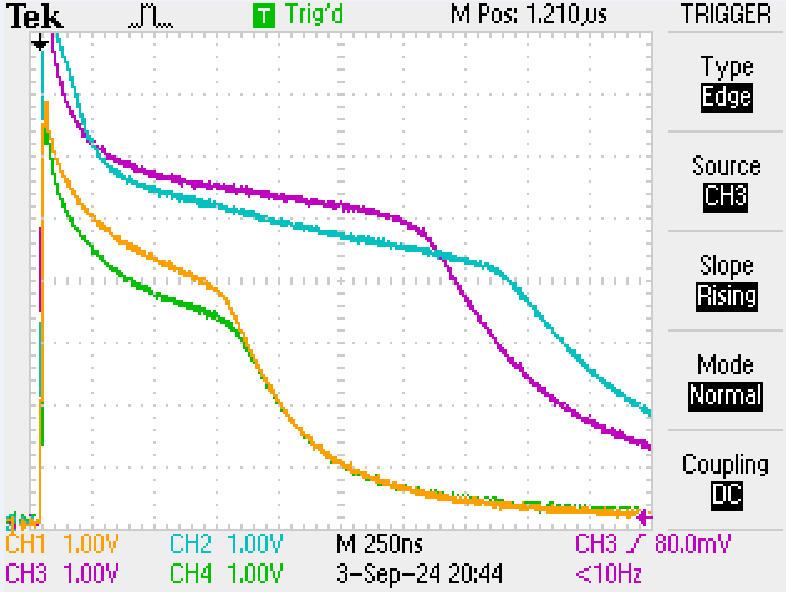
\includegraphics[width=0.7\textwidth]{figuras/3_señalesfotodiodos.png}
  \caption{Señal de salida de los cuatro fotodiodos del circuito de sintonización. (Fuente: elaboración propia).}
  \label{fig:senal_pico}
\end{figure}

Por lo tanto, la información relevante de la señal de salida de cada fotodiodo es su valor de pico, magnitud que debe ser detectada y digitalizada para permitir el control de sintonización.